\documentclass[../Main/Main.tex]{subfiles}
\begin{document}
Como base fundamental de este trabajo, a continuación y de forma preliminar, se presenta una visión general modelo, mientras que el resto del capítulo se enfocará en profundizar en cada parta que lo compone.\footnote{La versión completa del modelo se presenta en la sección \ref{sec:ModFinal} de la página \pageref{sec:ModFinal}.} Al modelo, se le titula \textit{bayesian piecewise polynomial model (bpwpm)} por sus siglas en inglés. Se trata de seguir la notación usada en los libros \citet{hastie2008elements} y \citet{james2013introduction}. Asimismo, al comienzo de este trabajo se presenta un glosario de los símbolos y signos usados.

Se supone la siguiente estructura: $\{(y_i,\xni)\}_{i = 1}^n$ es el conjunto de datos observados independientes con $n$ el tamaño de la muestra donde, $y_i \in \{0,1\}$ son las variables de respuesta binarias, $\xni \in \mathcal{X}^d \subseteq \mathbb{R}^d$ las covariables o regresores\footnote{Se utiliza la convención de usar negritas para distinguir vectores $\xni = (x_{i,1},\ldots,x_{i,n})^t$} y $d \in \mathbb{N}$ la dimensionalidad de las covariables.\footnote{En el lenguaje de aprendizaje de máquina, es usual hablar de \textit{outputs} e \textit{inputs} para referirse a $y_i$ y $\xni$ respectivamente \autocite{alpaydin2014introduction}.} Estos datos se organizan y se representan en una tabla (o matriz) como la presentada en la tabla \ref{tab:datos}. En ella, cada fila $i = 1,\ldots,n$ representa una observación. La primer columna corresponde al vector de respuestas y las columnas subsecuentes $j = 1,\ldots,d$ representan una covariable. Es útil pensar en estas columnas como $d$ \textit{dimensiones} que contienen información que induce la clasificación binaria.
\begin{table}[h]
$$
\left[\begin{array}{c|c} 
y_1 & \mathbf{x}_1 \\ 
\vdots & \vdots \\ 
y_n & \mathbf{x}_n \end{array}\right] 
\quad = \quad
\left[\begin{array}{c|ccc} 
y_1 & x_{1,1} & \ldots & x_{1,d} \\ 
\vdots & \vdots & ~ & \vdots \\ 
y_n & x_{n,1} & \ldots & x_{n,d}
\end{array}\right]
$$
\caption{Estructura de los datos}
\label{tab:datos}
\end{table}

Asimismo, se define el espacio de covariables $\mathcal{X}^d$ como el producto cartesiano de los rangos de cada covariable $j$. Esta definición, está relacionada con los polinomios por partes $f_j$ que se estudian en la sección: \ref{sec:fj}. 
\begin{align*}
	\mathcal{X}^d &= \mathcal{X}_1\times\mathcal{X}_2\times\ldots\times\mathcal{X}_d\\
	&= [a_1,b_1]\times[a_2,b_2]\times\ldots\times[a_d,b_d] \subseteq \mathbb{R}^d \\ 
\text{ con } \quad  a_j &= \min\left\{x_{1,j}\, ,\ldots,x_{n,j}\right\} \quad \forall j = 1,\ldots,d \\
	b_j &= \max\left\{x_{1,j}\, ,\ldots,x_{n,j}\right\} \quad \forall j = 1,\ldots,d. \\
\end{align*}
\vfill

\pagebreak
\begin{definition} \label{def:BPWPMPrelim}
El modelo bpwpm (preliminar), $\forall i = 1,\ldots,n$: 
\begin{align}
y_i &= 
	\begin{cases}
		1 & \iff \enspace z_i > 0 \\									0 & \iff \enspace z_i \leq 0
	\end{cases} \label{ec:DefY-Z} \\[2pt]
z_i\,|\,\xni\, &\sim \mathcal{N}(z_i\,|\,\eta(\xni),1) \label{ec:DefZ-X} \\[2pt]
\eta(\xni) &= f_0 + f_1(x_{i,1}) + f_2(x_{i,2}) + \ldots + f_d(x_{i,d}) \label{ec:etapred} \\[4pt]
f_j(x_{i,j}) &= \sum_{l = 1}^{\N} \beta_{j,l} \Psi_l(x_{i,j}, \mathcal{P}_j) \quad \forall j = 1,\ldots,d \label{ec:fj}
\end{align}	
\end{definition}
Las expresiones \eqref{ec:DefY-Z} y \eqref{ec:DefZ-X} introducen $n$ variables latentes $z_i$ independientes entre si con distribución normal. Estas variables se relacionan de forma unívoca con las respuestas $y_i$ formando una clase de equivalencia entre la probabilidad de dos eventos, permitiendo que se asocie el soporte binario de $y_i$ con el soporte real de $z_i$. Es decir, \eqref{ec:DefY-Z} y \eqref{ec:DefZ-X} implican:
\begin{align}
	P(y_i = 1 |\xni) = P(z_i > 0 \,|\, \xni) = \Phi(\eta(\xni)). 	\label{ec:IdentidadGLM}
\end{align}
Esta definición, \citet{albert1993bayesian}, es equivalente a la definición de un modelo probit pues la función liga resulta en la función de acumulación normal estándar $\Phi:\mathbb{R}\rightarrow (0,1)$ (Sección \ref{sec:GLM}). La identidad anterior \eqref{ec:IdentidadGLM} es inducida por la demostración de equivalencia entre definiciones que se detalla en el Teorema \ref{teo:Defs}. Una de las razones para adoptar esta perspectiva es que \citeauthor{albert1993bayesian} desarrollaron un método numérico vía simulación, bajo el paradigma bayesiano, para el cómputo exacto de las distribuciones posteriores del vector de parámetros $\betabf$ el cual resultaba atractivo para los objetivos del trabajo.
 
Posteriormente, la ecuación \eqref{ec:etapred} especifica la media de las variables latentes $z_i$, es decir, se le da forma funcional a $\E[z_i|\xni] = \eta(\xni)$. A esta función $\eta:\mathbb{R}^d\rightarrow\mathbb{R}$ se le conoce como función de predicción. La idea es suponer que la relación entre los componentes de las covariables $j = 1,\ldots,d$, es modelable como la suma de funciones (usualmente suaves) $f_j$ más un término independiente $f_0$. Esta definición corresponde a losmModelos  aditivos generalizados (GAM), una serie de modelos agrupados en \citet{hastie1986generalized}. En la sección \ref{sec:FuncPred} se presenta una introducción a ellos.

Finalmente, la expresión \eqref{ec:fj} define a las funciones $f_j \quad \forall j$ en la parte más profunda del modelo. Estas funciones $f_j: \mathcal{X}_j = [a_j,b_j] \rightarrow \mathbb{R}$ realizan una transformación no lineal de las covariables $x_{i,j}$. Este proceso se lleva a cabo mediante una expansión en bases funcionales revisada en la sección \ref{sec:fj}. El objetivo de esta expansión es expresar cada $f_j$ de una forma flexible, a través de la suma ponderada de funciones bases $\Psi_{j,l}(x_{i,j},\P_j)$ y parámetros desconocidos $\beta_{j,l}$ los cuales se deben de estimar. Asimismo, las funciones bases dependen de tres componentes: las covariables $x_{i,j}$, una partición $\P_j$ para cada dimensión\footnote{Definida sobre el intervalo $\mathcal{X}_j = [a_j, b_j] \quad \forall j = 1,\ldots,d$} y el número total de funciones base $\N\in\mathbb{N}$. Sus formas funcionales, no son más que truncamientos de orden mayor en las covariables, por ejemplo: $(x_{i,j} - a)_+^b$ con $a,b$ constantes definidas por $\N$ y $(\cdot)_+$ la función parte positiva, dando lugar a una expansión en  
polinomios por partes; particularmente, la presentada en \citet{mallik1998automatic}. Por el momento, se deja a las funciones bases $\Psi_{j,l}$ no especificadas por completo pues se decide presentarlas de forma constructiva en la sección \ref{sec:PolisYSplines}, derivando en su forma funcional final en las ecuaciones \eqref{ec:ExpBase_NEstrella} y \eqref{ec:PoliMallik}.

Para esclarecer un poco más el trabajo, en la figura \ref{fig:DiagramaMod} se presenta un diagrama del modelo y sus componentes. De izquierda a derecha y para toda $i=1,\ldots,n$: se busca transformar de forma no lineal a cada una de las covariables observadas $x_{i,j} \quad \forall j = 1,\ldots,d$ a través polinomios por partes condensados en las funciones $f_j$. Estas transformaciones dependen de parámetros desconocidos $\beta_{j,l}$ con $l =1,\ldots,\N$ y la partición de cada dimensión $P_j$. Una vez se tienen las covariables transformados, se suman las funciones $f_j$ con un intercepto local $f_0$ para obtener una función de predicción $\eta$. Esta función actúa como la media de la variable latente $z_i$ que relaciona a la respuesta $y_i$ con $\xni$. La relación se realiza a través de la función $\Phi$ para lograr la clasificación binaria en $y_i$. 
% Diagrama del modelo
\begin{figure}[h] 
\centering
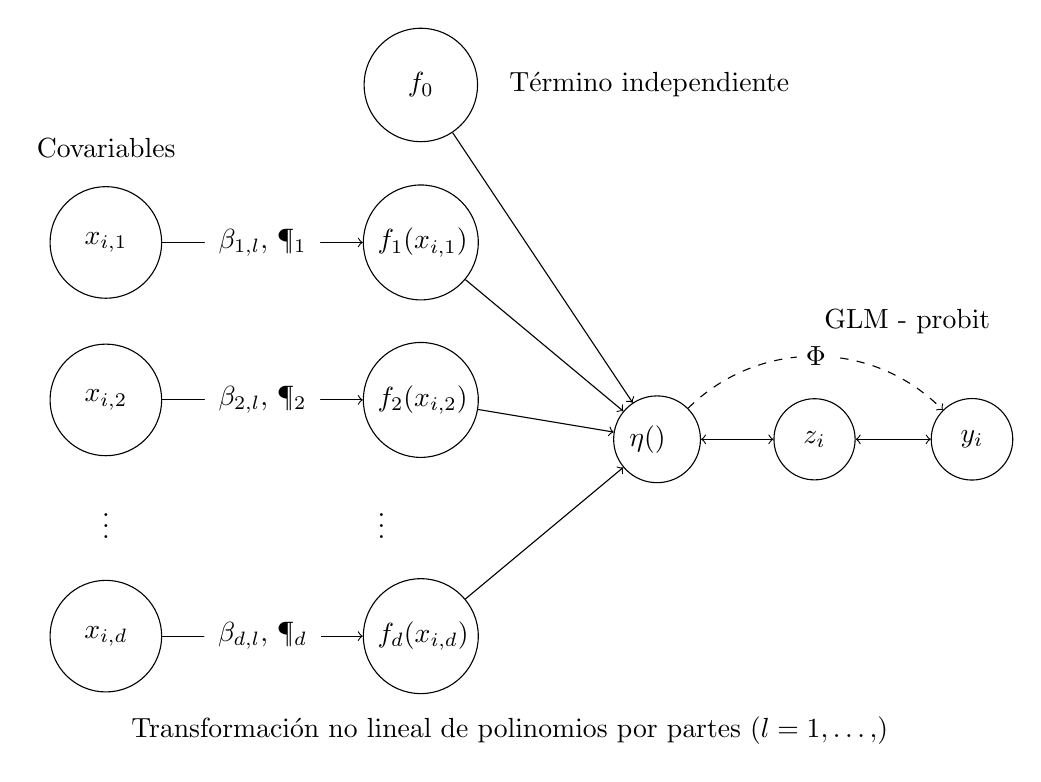
\begin{tikzpicture}
% Nodos Input
\begin{scope}[
		every node/.style = {shape = circle, draw = black,
			minimum size = 10mm,
			text width = 11mm, align = center}]
	\node (x1) at (0,6) {$x_{i,1}$};
	\node (x2) at (0,4) {$x_{i,2}$};
	\node[draw = white]     at (0,2.5) {$\vdots$};
	\node (xd) at (0,1) {$x_{i,d}$};

% Nodos Segunda Capa
	\node (f1) at (4,6) {$f_1(x_{i,1})$};
	\node (f2) at (4,4) {$f_2(x_{i,2})$};
	\node[draw = white]     at (3.5,2.5) {$\vdots$};
	\node (fd) at (4,1) {$f_d(x_{i,d})$};
	\node (f0) at (4,8) {$f_0$};
\end{scope}
	
% Nodos Lineales
\begin{scope}[
		every node/.style = {shape = circle, draw = black,
			minimum size = 7mm,
			text width = 7mm, align = center}]
\node (eta) at (7,3.5) {$\eta(\xni)\quad$};
\node (z) at (9,3.5) {$z_i$};
\node (y) at (11,3.5) {$y_i$};
\end{scope}

% Nodos Texto 
\node[right] at (-1,7.2) {Covariables};
\node[right] at (0.2,-0.2) {Transformación no lineal de polinomios por partes ($l = 1,\ldots,\N$)};
\node[right] at (9,5) {GLM - probit};
\node[right] at (5,8) {Término independiente};

% Pahts x a f_j y f_j a eta
\begin{scope}[
		every node/.style={fill = white, circle},
	    every edge/.style={draw = black, ->}]
	 
	% Paths x a f_j
	\path (x1) edge node {$\beta_{1,l}, \, \P_1$} (f1);
	\path (x2) edge node {$\beta_{2,l}, \, \P_2$} (f2);
	\path (xd) edge node {$\beta_{d,l}, \, \P_d$} (fd);

	% Paths f_j a f
	\path (f0) edge (eta);	
	\path (f1) edge (eta);
	\path (f2) edge (eta);
	\path (fd) edge (eta);
\end{scope}

% Ultimos Paths
	\path[->, dashed] (eta) edge [bend left = 45]
	node [fill = white] {$\Phi$}(y);	
	\draw[<->] (y) -- (z);	
	\draw[<->] (z) -- (eta);
\end{tikzpicture}
\caption{Diagrama del modelo}
\label{fig:DiagramaMod}
\end{figure}

Las aparentemente complejas interacciones entre todos los componentes del modelo no son más que respuestas estructurales a un proceso de \textit{síntesis} de la información. El modelo está buscando un patrón en las covariables $\xni$ para la correcta clasificación de su respuesta binaria asociada $y_i$. Este proceso, se lleva a cabo mediante tres transformaciones $f_j(x_{i,j}) \; \forall j$, $\eta(\xni)$ y finalmente $\Phi(\eta(\xni))$ las cuales cumplen el propósito de ir colapsando dimensiones. Se espera que este proceso, logre separar de forma flexible el espacio $d$-dimensional $\mathcal{X}^d$ a regiones más identificables (para la clasificación) que las regiones originales; donde finalmente, se le asigne una probabilidad a cada región de clasificación mediante $\Phi$. El Capítulo \ref{cap:EjYRes} cuenta con visualizaciones que esperan volver estos conceptos teóricos en algo más concreto. 

Antes de continuar, vale la pena mencionar el precepto de \citet{box1976science}:
\begin{quote}
\textit{All models are wrong but some are useful}
\end{quote}
En la perspectiva del autor, no se está tratando de construir un modelo que replique el proceso generador de los datos. Más bien, se está tratando de construir una útil abstracción de la realidad a través de un modelo matemático. Escoger cualquier enfoque de modelado, es un proceso reduccionista y por ende, falible. Sin embargo, no significa que no se puedan discernir patrones en los datos y aprender de ellos. 

\section{Modelos lineales generalizados (GLM)} \label{sec:GLM}
Los modelos lineales generalizados (GLM), \citet{maccullagh1989generalized}, surgen como una generalización del modelo de regresión lineal:
\begin{align*}
	y_i|x_i &\sim \mathcal{N}(\mu(\xni), \sigma^2)  \quad \forall i = 1,\ldots,n\\
	\mu(\xni) &= \beta_0 + \tilde{\betabf}^t\xni,
\end{align*}
donde $y_i \in\mathbb{R}$, $\tilde{\betabf} \in \mathbb{R}^{d}$ es un vector de parámetros y $\mu(\xni) = \E[y_i|\xni]$.\footnote{Se usa $\tilde{\betabf}$ para distinguir al vector de dimensionalidad $d$ y a $\betabf$ para distinguir al vector que contiene el término independiente, es decir, $\betabf\in \mathbb{R}^{d+1}$} Las regresiones lineales, están acotadas a datos donde la variable de respuesta $y_i$ tenga soporte real. En consecuencia se desarrollan los GLM, que busca flexibilizar este soporte a una mayor cantidad de respuestas. Esta modificación vuelve al modelo más complejo y deriva en diversas técnicas para la estimación de $\betabf$. Asimismo, la generalización del modelo lleva a que la intrepretación de los parámetros no sea trivial.\footnote{Por ejemplo, en un modelo logit que busca la predicción de variables binarias, se logra expresar el logaritmo de la proporción de probabilidades (\textit{Log-Odds-Ratio}) como una combinación lineal de las covariables. $\ln(p_1 / p_0) = \betabf^t x$, donde $p_k$ con  $k = \left\{0,1\right\}$, es la probabilidad de que la respuesta $y$ sea $0$ o $1$ respectivamente.}\\

\begin{definition} El modelo lineal generalizado, \citet{sundberg2016exponential}:
\begin{align} 
	y &\sim F(\mu(\xsn)) \label{ec:GLM} \\ 
	\eta &= \beta_0 + \betabf^t\xsn \nonumber \\ 
	g(\mu) &= \eta \nonumber
\end{align}
\end{definition}
cuenta con los siguientes tres elementos:
\begin{itemize}[label={}]
	\item $F$: distribución de la familia exponencial que describe el dominio de las respuestas $y$, cuya media $\mu(\cdot)$ es dependiente de las covariables.\footnote{Al trabajar con distribuciones de la familia exponencial es usual parametrizar la distribución no con la media $\mu$ sino con el parámetro canónico $\theta$.} Por ejemplo: Bernoulli si $y$ es binaria, Poisson si $y \in \mathbb{Z}^+$ o una distribución Gamma si $y \in \mathbb{R}^+$
	\item $\eta$: predictor lineal que explique (linealmente) la variabilidad sistemática de los datos.%\footnote{Como restricción adicional, en el modelo clásico se pide que $\text{dim}(\beta) = d < n.$}
	\item $g$: función liga que une la media $\mu$ de la distribución con el predictor lineal,\footnote{Si la función $g$ es tal que $\eta \equiv \theta$ entonces se dice que $g$ es la función liga canónica. } es decir: $g(\mu(x)) = g(\E[y|x]) = \betabf^tx$. $g$ puede ser cualquier función monótona que idealmente mapee de forma suave y biyectiva el dominio de la media $\mu$ con el rango del predictor lineal $\eta$ \autocite{hardle2004semiparametric}. 
\end{itemize}

\subsection{El modelo probit}
Por lo pronto, la discusión se centrará en la distribución Bernoulli pues resulta de forma natural dado que se busca construir un clasificador supervisado donde las respuestas observadas sean binarias, i.e. $y_i \in \{0,1\} \; \forall i=1,\ldots,n$. Esto es:
\begin{align}
	y_i \sim \Be(y_i \, |\, p_i). \label{ec:ModBernoulli}
\end{align}
La distribución Bernoulli (\ref{ec:ModBernoulli}) tiene una estructura sencilla que puede ser resumida en las siguientes expresiones $\forall i = 1,\ldots,n$:  
\begin{align}
	f(y_i|p_i) &= p_i^{y_i}(1 - p_i)^{1 - y_i} \label{ec:DensidadBernoulli} \\
	\text{donde }\, y_i &\in \{0,1\},  \nonumber\\
	\E[y_i] &= \mu_i = P(y_i = 1) = p_i  \nonumber\\
	\Var[y_i] &= p_i(1 - p_i) \nonumber. 
\end{align}			
%&= \exp\left\{y_i\ln\left(\frac{p_i}{1 - p_i}\right) + \ln(1-p_i)\right\} \label{ec:DensidadBernoulliCanon} \\

En (\ref{ec:DensidadBernoulli}) se observa la función de masa de probabilidad Bernoulli en su forma tradicional que puede ser reexpresada para que cumpla la definición de la familia exponencial.\footnote{Una distribución (de un solo parámetro) se dice que pertenece a la familia exponencial si se puede expresar de la forma: $f(y;\theta) = h(y)\,\text{exp}\left\{y\cdot\theta - A(\theta)\right\}$ con $h(y)$, $A(\theta)$ funciones conocidas y $\theta$ el parámetro canónico, en el caso Bernoulli: $\theta(p) = \ln p/(1-p)$.} Dado el soporte y la definición de la distribución Bernoulli, la media de la distribución $\mu = p$ coincide con la probabilidad de que la variable aleatoria tome el valor de uno. Asimismo, la varianza queda especificada por el mismo parámetro $p$. 

El que la media conocida con la probabilidad de éxito en una distribución Bernoulli es de gran utilidad en un contexto de clasiicación por varias razones. Primero, al modelar la media $\mu = p$, se está caracterizando por completo la distribución y la predicción de la variable $y$. Segundo, se restringen las posibles funciones liga a las funciones que mapeean de forma biyectiva $\mathbb{R}$, el dominio del predictor lineal $\eta$, al el rango de la media, el intervalo $(0,1)$. Dadas las propiedades buscadas, es usual usar como función liga a las inversas de funciones \textit{sigmoidales}. Las funciones sigmoidales, son funciones \linebreak $s:\mathbb{R}\rightarrow (0,1)$ estrictamente monótonas y por ende, biyectivas. Algunos ejemplos son la ya mencionada logit, la función probit que concierne a este trabajo o la curva de Gompertz. Estas funciones cumplen un papel de activación, es decir, una vez que el predictor lineal rebase cierto umbral, crecen rápidamente y toman valores más cercanos a uno, \textit{activando} así la probabilidad de que $y$ sea uno.\footnote{En un contexto de aprendizaje de máquina, se les conoce como funciones de activación a las inversas de la funciones liga $g^{-1}$ que no necesariamente tienen que ser biyectivas \autocite{bishop2006pattern}. Por ejemplo, en redes neuronales es común utilizar la función $\textit{ReLu}(x):= \max\left\{0,x\right\}$ la cual no es suave \autocite{3blue1brown2017}.}

En particular, en este trabajo se escoge como función liga a la función probit dándole nombre al modelo, en consecuencia al trabajo de \citet{albert1993bayesian}. La función probit la inversa de la función de acumulación normal estándar $\Phi(\cdot)$, i.e. $g(\mu) = g(p) = \text{probit}(p) = \Phi^{-1}(p)$. Dado que la notación puede ser confusa, en la figura \ref{fig:DiagramaFuncLiga} se presenta una representación gráfica de la función liga para un modelo probit.\footnote{Para no caer en redundancia de notación se tiene a partir de ahora: $s(x) = g^{-1}(x) = \Phi(x)$ la función de acumulación normal estándar. Asimismo, se deja de usar $\mu$ para referirse a la media y se utiliza únicamente $p$.}

% Diagrama de g
\begin{figure}[h]
\centering
\begin{tikzpicture}
% Flechas (circulo) (s para demostrar que el orden importa en rikz
%\draw [black] (0,0) circle [radius = 2];
% Dibujo nodos
\begin{scope}[
		every node/.style = {fill = white, shape = rectangle }]
		
	\node (g) at (0,1.5) {$g(p)$};
	\node (ginv) at (0,-1.5) {$g^{-1}(\eta)$};
	\node (R) at (1.5,0) {$\eta \in \mathbb{R}$};
	\node (int) at (-1.5,0) {$p \in (0,1)$};
	
\end{scope}

% Flechitas
\begin{scope}[
		every node/.style={fill = white, circle},
	    every edge/.style={draw = black, ->}]
	
	\path (g) edge [bend left] node [above right] 
	{e.g. $\Phi^{-1}(p)$} (R);
	\path (R) edge [bend left] (ginv);
	\path (ginv) edge [bend left] node [below left] {e.g. $\Phi(\eta)$} (int);
	\path (int) edge [bend left] (g);
	
\end{scope}

\end{tikzpicture}
\caption{Esquema de función liga $g$ para un modelo probit}
\label{fig:DiagramaFuncLiga}
\end{figure}

Juntando todos los componentes, se está en posibilidades de detallar el modelo probit en su forma más rigurosa. Rescatando la notación de un GLM \eqref{ec:GLM} con sus respectivas covariables $\xni$: 
\begin{align}
y_i|\xni & \sim \Be(y_i|p_i) \qquad \forall i = 1,\ldots,n\label{ec:ModProbitA}\\
\eta_i &= \eta(\xni) \label{ec:ModProbitB} \\
p_i &= \Phi(\eta_i) = \Phi(\eta(\xni)) \label{ec:ModProbitC}
\end{align}

\subsubsection*{Equivalencia en las definiciones del modelo}
El lector notará, que la especificación del modelo probit en las ecuaciones anteriores no corresponde a la definición mostrada al principio del capítulo. No obstante, las definiciones son equivalentes y se prueba a continuación.\\

\begin{theorem} \label{teo:Defs}
Un modelo probit especificado en \eqref{ec:ModProbitA} y \eqref{ec:ModProbitC}, es equivalente a un modelo de variable latente como el presentado en \eqref{ec:DefZ-X} y \eqref{ec:DefY-Z}.
\end{theorem}

\begin{proof} Dado un modelo probit se tiene, sin perdida de generalidad $\forall i = 1,\ldots,n$:
\begin{align*}
	\E[y_i\,|\,\xni] &= p_i  \\
				&= P(y_i = 1\,|\,\xni)  \qquad \text{por \eqref{ec:ModProbitA}}\\
				&= \Phi(\eta(\xni)) \qquad \text{por \eqref{ec:ModProbitC}}
\end{align*}
Lo cual, es equivalente a introducir $n$ variables aleatorias $\tilde{z}_i \sim \mathcal{N}(\tilde{z}_i|0,1)$ tales que:
\begin{align*}
	\Phi(\eta(\xni)) 	&= P(\tilde{z}_i \leq \eta(\xni)\,|\,\xni)
					\quad \text{por definición de la función de acumulación}\\
			      	&= P(\tilde{z}_i > - \eta(\xni)\,|\,\xni) \quad \text{por simetría de la distribución normal}\\
			      	&= P\left(\dfrac{\tilde{z}_i + \eta(\xni)}{1} > 0\,\bigg|\,\xni\right)\\
			      	&= P(z_i > 0\,|\,\xni).
\end{align*}
Donde $z_i = \tilde{z_i} + \eta(\xni)$ es una transformación biyectiva de $\tilde{z}_i$ tal que: 
$$z_i|\xni \sim \mathcal{N}(z_i|\eta(\xni),1),$$ 
lo cual es idéntico a la expresión \eqref{ec:DefZ-X}. Asimismo, al tener la igualdad $$P(y_i = 1|\xni) = P(z_i > 0|\xni)$$ y por ende su probabilidad complementaria $P(y_i = 0|\xni) = P(z_i \leq 0|\xni)$, se define una clase de equivalencia entre probabilidades. Es decir, se puede definir $y_i$ en términos de $z_i$ y viceversa, dando lugar a la definición \eqref{ec:DefY-Z}. 

El argumento es casi idéntico si la demostración se comienza asumiendo la definición de un modelo de variable latente como en \eqref{ec:DefZ-X} y \eqref{ec:DefY-Z} y se construye hasta llegar a un GLM como en  \eqref{ec:ModProbitA} y \eqref{ec:ModProbitC}. Sin embargo, se tiene la peculiaridad de que la varianza debe de ser igual a uno para ser que la correspondencia entre definiciones sea exacta.\footnote{Comenzar con $z_i|\xni \sim \mathcal{N}(z_i|\eta(\xni),\sigma^2)$ con $\sigma^2\neq 1$ deriva en que $p_i = \Phi(\eta(\xni)/\sigma)$ lo cual es diferente a lo que se tiene en \eqref{ec:ModProbitC}.}
\end{proof}

La ecuación \eqref{ec:ModProbitB} realmente no influye en la prueba pues esta puede tener la forma funcional que se requiera para la aplicación especifica, ya sea lineal $\eta_i = \beta_0 + \betabf^t\xni$ como en \eqref{ec:GLM} o algo diferente como se opta en este trabajo.

\subsection*{Liga entre la variable latente $z$ y $\eta$} \label{sec:VarLat}
Para entender como se conectan las $n$ variables latentes $z_i$ con sus respectivos predictores lineales $\eta(\xni)$, se necesita profundizar un poco más en el objetivo del modelo. Recapitulando, mediante la función liga $\Phi$ se une la media $p_i$, la probabilidad de que la respuesta $y_i$ sea uno con los datos $\xni$. Esto se logra, a través de una variable latente $z_i$ definida con distribución normal cuya media $\eta(\xni)$, la función de predicción, es una transformación de las covariables $\xni$. Es decir,
\begin{align} \label{ec:RegMedia}
	P(z_i > 0|\xni) = P(y_i = 1|\xni)= p_i(\xni) &=\E[y_i|\xni] = g^{-1}(\eta(\xni)) = \Phi(\eta(\xni)).
\end{align}
Este enfoque funciona, además de por el componente algorítmico, por la siguiente idea. Si se quiere crear una regla de decisión que clasifique observaciones en categorías binarias con base en cierta información, parecería intuitivo condensar esa información de forma que proporcione suficiente evidencia para inducir la clasificación. Traduciendo en términos matemáticos, la información $\xni$ se condensa en la función $\eta(\xni)$ la cual induce la clasificación de $y_i$ a través de la ecuación \eqref{ec:RegMedia}. Por ejemplo, si se tiene una $\eta(\xni)>>0$ para alguna observación $i$, implicaría que $P(z_i > 0|\xni)$ es cercano a uno (por el dominio de $\Phi$) y por lo tanto, es muy probable que $y_i$ sea un uno. El argumento es idéntico para la probabilidad complementaria.

Al final, como se menciona anteriormente, el modelo está resumiendo información al ir colapsando dimensiones. El siguiente paso en el modelo consiste en detallar la transformación que debe realizar el predictor lineal $\eta(\xni)$. Tradicionalmente como se mencionó en \eqref{ec:GLM}, esta transformación era lineal tanto en parámetros como en covariables, dando lugar a fronteras de decisión lineales. Sin embargo, el siguiente paso lógico es modificar estos modelos para que las fronteras puedan ser más flexibles, rompiendo la linealidad en las covariables para lograr encontrar patrones más complejos. 

\section{La función de predicción $\eta$} \label{sec:FuncPred} 
\subsection{Una breve introducción a los GAM}
Como se detalla en la página 6 de \citet{james2013introduction}, conforme avanzaron los métodos y el poder computacional disponible se fueron desarrollando técnicas cada vez más poderosas que permitieron romper la linealidad en las covariables. En particular, \citeauthor{hastie1990generalized} se agrupan una clase de modelos a los que se les da el nombre de modelos aditivos generalizados (GAM). Estos modelos logran identificar relaciones no lineales utilizando, usualmente, métodos no paraméticos de suavizamiento en los datos  adoptando así, un enfoque de \textit{dejar que los datos hablen por si mismos}.\footnote{Página 1 de \citet{hastie1990generalized}}\\

\begin{definition} \label{def:GAM}
Un GAM, tiene la forma $\forall i =1,\ldots,n$:
\begin{align}
	\E[y_i|\xni] = g^{-1}\left[f_0 + f_1(x_{i,1}) + \ldots + f_d(x_{i,d})\right],\label{ec:GAM}
\end{align}
con $g^{-1}$ la inversa de la función liga definida en \eqref{sec:GLM} y el predictor lineal $\eta(\xni) = f_0 + f_1(x_{i,1}) + \ldots + f_d(x_{i,d})$. 
\end{definition}

La idea fundamental de los GAM, es asumir que los efectos en las covariables se pueden modelar como una suma de funciones por componentes, es decir, cada covariable $x_j \quad \forall j =1,\ldots,d$ está siendo transformada de forma no lineal e independiente por una función asociada $f_j \quad \forall j$. De esta forma, se retiene algo de la interpretabilidad del modelo lineal. La funciones $f_j$ que ahora componen el predictor lineal $\eta$ se busca que sean tan flexibles como sea necesario, permitiendo que el estadista pueda hacer menos suposiciones rígidas sobre los datos. Estas funciones $f_j$ son suaves y no especificadas (\textit{no paramétricas}), es decir, no tienen una forma funcional concreta y representable algebraicamente. Sin embargo, es justamente ahí donde recae la fuerza de los GAM: al dejar a las funciones $f_j$ ser no especificadas, se permite que estas capturen los efectos necesarios en los datos para hacer el mejor ajuste posible, a este proceso se le llama suavizamiento. 

Un suavizador, se puede definir de forma general, como una herramienta que resume la tendencia de la respuesta $y$ como función de las covariables $\xsn$ y produce un estimador $f$ que es menos variable (ruidoso) que la respuesta en si. Como se mencionó con anterioridad, estos suavizadores son de naturaleza no paramétrica pues no se asume una dependencia rígida de $y$ en $\xsn$.\footnote{Las técnicas no paraméticas están fuera del alcance de este trabajo. Sin embargo, vale la pena una mención especial por su funcionalidad, practicalidad y forma intuitiva, además del sinfín de aplicaciones que tienen. Una guía comprensiva de estas se encuentra en el libro \citet{wasserman2007all}.} Como ejemplos prácticos de métodos no paramétricos, se encuentran los ajustes de medias móviles y el suavizamiento LOESS\footnote{El suavizamiento LOESS, \textit{locally estimated scatterplot smoothing}, es un tipo de regresión local que ajusta modelos más simples a subconjuntos de los datos para construir una función global que describa de forma no lineal la variabilidad intriseca que se presenta.} \autocite{cleveland1988locally}. 

En un GAM la estimación de las funciones $f_j$, se lleva a cabo por el algoritmo de ajuste hacia atrás (\textit{backfitting algorithm}), \citet{hastie1986generalized}. Este procedimiento, busca dar estimadores de cada $f_j$ de forma iterativa por componentes, utilizando como regresores los residuales parciales. Por ejemplo, sea $d = 2$ y $g^{-1}(w) = w$ la función identidad, quedando así el modelo:
$$\E[y_i|\xni] = f_0 + f_1(x_1) + f_2(x_2).$$
Dados estimadores preliminares $\hat{f}_0$ y $\hat{f}_1$ de las respectivas funciones $f_0$ y $f_1$, se definen los residuales parciales: $\E[y_i|\xni] - (\hat{f}_0 + \hat{f}_1(x_1))$ sobre los cuales se busca suavizar $f_2$. Este proceso resulta en una mejor estimación de la función $f_2$, con la cual, se puede mejorar el estimador de $f_1$. Ese proceso se lleva a cabo de forma iterativa, hasta que el cambio en las funciones funciones $f_j$  sea menor que un umbral especificado.\footnote{La demostración de convergencia de un GAM se encuentra en \citet{stone1985additive}} Este algoritmo, se puede extender para $d$ y $g$ arbitrarias y es bastante flexible a modificaciones. En un GAM, las curvas resultantes de las funciones $f_j$ son suaves y lejos de ser lineales. Asimismo, sus formas, pueden ayudar a entender el fenómeno subyacente. 

\subsubsection*{Los GAM en el contexto de este trabajo}
Sin dudar la elegancia y practicalidad de los métodos no paramétricos, para este trabajo, se opta modificar el enfoque original de los GAM y darles una forma rígida a las funciones $f_j$, regresando a los dominios de la estadística paramétrica. Esta decisión, pues se busca profundizar en los polinomios por partes estudiados en la siguiente sección \ref{sec:fj} que componen a las funciones $f_j$. Aunque pareciera una desviación considerable del trabajo original de \citeauthor{hastie1990generalized}, en realidad en el Apéndice \ref{ap:Splines} se detalla como los polinomios por partes son el resultado de plantear la idea de suavizamiento como un problema de optimización. Asimismo, los GAM son tan flexibles en su definición (y concepto) que es usual restringir las funciones $f_j$ con formas funcionales concretas.\footnote{Capitulo 9.1 y Ejemplo 5.2.2 de \citet{hastie2008elements}}

Bajo esta óptica, para este trabajo se retienen dos de las ideas fundamentales de los GAM: aditividad y las transformaciones por componentes de las covariables. Es decir, la definición de un GAM \eqref{ec:GAM} sustituye el predictor lineal tradicional de los GLM \eqref{ec:GLM}, $\eta(\xni) = \beta_0 + \tilde{\betabf}^t\xni$, con una suma de funciones $\sum_j^d f_j(x_j)$ más un intercepto constante $f_0$ que juega el papel de $\beta_0$, dando lugar a la ecuación \eqref{ec:etapred} definida a inicios de este capítulo:
\begin{align}
\eta(\xni) &= f_0 + f_1(x_{i,1}) + f_2(x_{i,2}) + \ldots + f_d(x_{i,d}). \tag{\ref{ec:etapred}}
\end{align}
Se hace notar, que a diferencia de los modelos lineales donde se tiene a los parámetros $\betabf$ incluidos en la expansión de $\eta$,  en los GAM los parámetros se incluyen dentro de cada una de las $f_j$ pues, los efectos de cada covariable son resumidos dentro de las mismas transformaciones. Aunque se pueden agregar parámetros que ponderen cada $f_j$, sobre-parametrizar puede llevar a la incorrecta especificación del modelo y caer en problemas de identificabilidad de los parámetros.

Al entender que cada $f_j$ es una transformación no-lineal de $x_j$ (como lo sería una transformación logarítmica o una transformación Box-Cox) se le regresa cierta interpretabilidad al modelo. Es decir, cada $f_j(x_{i,j})$ es el efecto que tiene la covariable $j$, para una observación $i$, en la clasificación. Por lo tanto y heredado de la ecuación \eqref{ec:RegMedia} si $f_j$ es más positiva para esta observación $i$, se tiene mayor evidencia (en el componente $j$) de que la respuesta binaria asociada $y_i$ sea uno. En la peculiaridad de que $d = 2$, se podrá visualizar, no solo las funciones $f_j$ de manera independiente, sino toda $\eta(\xni)$ en $\mathbb{R}^3$ como una serie de picos y valles donde será positiva en caso de que $y_i $ sea clasificada como uno y  negativa en caso de que sea cero. La imagen de la página \pageref{fig:YY3D}.

La inclusión de un término independiente $f_0$ es importante en los GAM pues es uno de los resultados de la derivación mencionada en el apéndice \ref{ap:Splines}. Asimismo, se debe considerar el caso tal que $f_j(x_j)=0\quad\forall j$ de donde se necesita un término independiente $f_0$. Para este trabajo al término $f_0$ se le da el mismo tratamiento que el de un parámetro independiente convencional, por lo tanto, se estima usando el mismo procedimiento que todos los demás parámetros. Este hecho se esclarecerá en las secciones subsecuentes. Las imágenes \ref{fig:T1M1F1} y  \ref{fig:T1M1F1} de la página \pageref{fig:T1M1F1}, son solo algunos ejemplos de las posibles formas finales que pueden adoptan las funciones $f_j$. Para esta realización particular del modelo, están compuestas por segmentos de recta que no son suaves.

\section{Funciones $f_j$} \label{sec:fj}
Finalmente se trata la parte más profunda del modelo, las funciones $f_j$  que, como se mencionó anteriormente, son transformaciones no lineales de cada componente $x_j$. Lo que buscan es suavizar la nube de datos, para posteriormente sumarlas entre si y dar una media $\eta$ que resuma toda la información en un número real. Como se menciona en la introducción de \citet{hardle2004semiparametric}, el suavizamiento de los datos es central en la estadística inferencial. La idea es extraer la señal entre el ruido y para ello, se intenta estimar y modelar la estructura subyacente. Este suavizamiento, se llevará a cabo usando una expansión en bases funcionales, particularmente el tipo de polinomios por partes presentados en \citet{mallik1998automatic}. Toda la siguiente sección se concentra en darle forma funcionales a las sub-funciones $\Psi$ para definir por completo $f_j$ y por ende $\eta$. 

\subsection{Expansión en bases funcionales}
Saliendo por un momento del domino de la estadística, se definen las expansiones en bases funcionales. Sin entrar mucho en los detalles técnicos, dado un espacio funcional\footnote{Espacio vectorial cuyos elementos son funciones.} se puede representar cualquiera de sus elementos, en este caso una función arbitraria $h$, como la combinación lineal de los elementos de la base $\Psi$  y constantes $\beta$. En particular (y dados los objetivos del trabajo) se considera el espacio funcional que mapea $\mathbb{R}^d$ a $\mathbb{R}$, quedando entonces la expansión: 
\begin{align} 
	h(\xsn) = \sum_{l = 1}^{N}\beta_l\Psi_l(\xsn) = \tilde{\beta}bf^t\Psi(\xsn). \label{ec:ExpansionBases}
\end{align}
Bajo esta definición, $\Psibf(\xsn) = (\Psi_1(\xsn),\ldots,\Psi_{N}(\xsn))^t$ es un vector cuyos elementos $\Psi_l(\xsn)$ son llamados funciones base y tienen el mismo mapeado que $h$. De la misma forma $\tilde{\betabf} = (\beta_1,\ldots,\beta_{N})^t$ es un vector de coeficientes constantes. Finamente, $N\in\mathbb{N}$ es un entero mayor o igual a la dimensión del espacio funcional que se maneja.\footnote{Dependiendo de el espacio funcional y la complejidad de la función real por estimar $h$, en ocasiones se requiere que $N = \infty$ para que se de la igualdad estricta \autocite{bergstrom1985estimation}.}

En un contexto estadístico de regresión, se definen los modelos lineales de bases funcionales,\footnote{\textit{Linear basis function models}.} capitulo 3 de \citet{bishop2006pattern}, como:
\begin{align} 
	h(\xsn) = \beta_0 + \sum_{l = 1}^{N} \beta_l\Psi_l(\xsn) = \beta_0 + \tilde{\betabf}^t\Psibf(\xsn), \label{ec:LBFM}
\end{align}
lo cual es idéntico a \eqref{ec:ExpansionBases} con la adición del término independiente $\beta_0$. Bajo este contexto, se busca representar una transformación $g$ de la media condicional de la respuesta por una función dependiente de los datos, es decir: $h(\xsn) = g(\E[y\,|\xsn]) = \eta(\xsn)$. Por lo tanto se puede pensar que esta función $h$ es análoga a la función de predicción $\eta$, también puede ser expresada como su expansión en bases funcionales.\footnote{Un supuesto fuerte pero útil.} 

La idea, es que se remplace (o se aumente) la cantidad de covariables $\xsn$ con transformaciones de estas, capturadas en el vector $\Psi(\xsn)$. Como ejemplos se pueden tener:
\begin{itemize}[label = {}]
	\item $\Psi_l(\xsn) = x_l \quad \forall\,l = 1,\ldots, N = d$,  recupera un GLM tradicional.
	\item $\Psi_l(\xsn) = \ln x_l$ ó $x^{1/2}_l$ para alguna $l = 1,\ldots, N = d$, donde se tienen transformaciones no lineales en cada una (o algunas) de las covariables.
	\item $\Psi_l(\xsn) = \exp\left\{-\dfrac{(x_l - \mu_l)^2}{2s^2}\right\} \quad l = 1,\ldots,d$ una expansión en bases gaussianas con $\mu_j$ el parámetro que gobierna la ubicación y $s$ la escala de las funciones bases.
	\item $\Psi_l(\xsn) = x_j^aI( \t_b \leq x_j <  \t_c)$ para alguna $j$ y $\forall l =1,\ldots,N$ con $a\in \mathbb{N}$ y $\tau_b$, $\tau_c$ nodos fijos. Dando lugar a  una expansión en bases polinómicas como la que se usa en este trabajo (sección \ref{sec:PolisYSplines}).
	\item $\Psi_l(\xsn) = x_jx_k  \quad \forall l = 1,\ldots,N,$  para alguna $j,k$. Da lugar a un modelo con interacciones. 
\end{itemize}

Como se ve, esta representación es tan flexible que engloba muchos de los modelos y transformaciones posibles en el mundo de las regresiones, uniendo temas de análisis funcional con estadística aplicada. Asimismo esta representación ha resultado ser de gran utilidad en la práctica. Se hace notar que el último ejemplo rompe con la aditividad inherente de los modelos que se han estudiado hasta ahora, mostrando que esta generalización no está restringida a ser completamente aditiva en covariables. Sin embargo $h$, por su construcción, siempre es lineal en los parámetros $\betabf$ pero no lineal en las covariables, dependiendo de la forma de $\Psi(\xsn)$.

Dependiendo del tipo de datos y el propósito del modelo, puede ser conveniente usar algún tipo de funciones base sobre otras. Sin embargo, sobre todo cuando se tiene poca o ninguna experiencia con los datos, se busca una representación flexible (por no decirla ingenua) de éstos. El método más común es tomar una familia grande de funciones que logre representar una gran variedad de patrones. No obstante, una desventaja de estos métodos es que al contar con una cantidad muy grande de funciones base y por ende parámetros, se requiere controlar la complejidad del modelo para evitar el \textit{sobre-ajuste}\footnote{Seguir los datos tan de cerca que se pierda la señal entre el ruido}. Algunos de los métodos más comunes para lograrlo son los siguientes, \citet{hastie2008elements}:
\begin{itemize}[label={}]
	\item Métodos de restricción: se selecciona un conjunto finito de funciones base y su tipo, limitando así las posibles expansiones. Los modelos aditivos como los usados en este trabajo, son un ejemplo de esto.  
	\item Métodos de selección de variables: como lo son los modelos CART y MARS,\footnote{\textit{Classification \& regression tree} \autocite{breiman1984classification} y \textit{multivariate adaptive regression splines} \autocite{friedman1991multivariate} respectivamente.} donde se explora de forma iterativa las funciones base y se incluyen aquellas que contribuyan a la regresión de forma significativa.
	\item Métodos de regularización: donde se busca controlar la magnitud los coeficientes, buscando que la mayoría de ellos sean cero, como los son los modelos \textit{Ridge} y  \textit{LASSO}.\footnote{\textit{Least absolute shrinkage and selection operator} \autocite{hoerl1970ridge, tibshirani1996regression}}
\end{itemize}

Para los objetivos de este trabajo, lo que se busca expresar en su expansión de bases funcionales no es la función de predicción $\eta$, sino sus componentes aditivos $f_j$. Al aislar cada función $f_j$ que dependen únicamente de una variable real $x_j \quad \forall j$, es decir: $f_j:\mathbb{R}\rightarrow\mathbb{R} \quad \forall j$, se puede simplificar la exposición y reducir el número de índices pues sus expresiones algebraicas son idénticas.

\subsection{Polinomios por partes y \textit{splines}} \label{sec:PolisYSplines}
Los polinomios por partes, por su flexibilidad, ha resultado ser de gran utilidad en diversas ramas de de las matemáticas. En particular, el mundo de la estadística surgen de forma natural como solución a varios problemas de modelado (ver apéndice \ref{ap:Splines}). Antes de exponer la representación final de las funciones $f_j$, se da una exposición constructiva de los polinomios por partes. Se usa como referencia las primeras dos secciones de el Capitulo 5 de \citet{hastie2008elements} y \citet{wahba1990splines}. 

Sea $x\in[a,b]\subseteq\mathbb{R}$, se busca separar $[a,b]$ en $J$ intervalos. Por lo tanto, se construye una partición correspondiente $\P = \left\{\t_1, \ldots,  \t_{J-1} \right\}$ tal que $a \leq  \t_1 < \ldots <  \t_{J-1} \leq b$. Las constantes $\t$ son llamadas \textit{nodos}.\footnote{En la definición, se puede incluir o no la frontera dependiendo de si se busca hacer inferencia fuera del intervalo acotado de los datos.} Con los nodos seleccionados, se puede representar a diferentes niveles de precisión una función arbitraria $h$, a través de su expansión análoga a la ecuación \eqref{ec:ExpansionBases}, donde cada $\Psi_j$ será una función que depende, tanto de la partición $\P$ como de la variable real $x$. 

Para ejemplificar se presenta un ejemplo sencillo. Primero, se parte el intervalo en tres pedazos ($J = 3$) definiendo una partición con dos nodos, es decir: $\P = \left\{\t_1,  \t_2\right\}$. Posteriormente, a cada subintervalo se le asocia una función $\Psi_j$ tales que:
\begin{align*}
	\Psi_1(x,\P) &= I( x <  \t_1) \\
	\Psi_2(x,\P) &= I( \t_1 \leq x <  \t_2) \\
	\Psi_3(x,\P) &= I( \t_2 \leq x ),
\end{align*}
con $I(\cdot)$ la función indicadora que vale uno si $x$ se encuentra en la región y cero en otro caso. Bajo esta definición, se construye una función $h$: 
\begin{align*}
		h(x) &= \sum_{l = 1}^J \beta_l\Psi_l(x) \\
			 &= \beta_1 I( x <  \t_1) + \beta_2 I( \t_1 \leq x <  \t_2) + \beta_3 I( \t_2 \leq x).
\end{align*}
Esta función $h$ es una función escalonada, en el sentido de que cada región de $x$ tiene un nivel $\beta_j$.\footnote{Dado un conjunto de observaciones $\{(y_i,x_i)\}_{i = 1}^n$, si se buscara estimar los parámetros $\beta$ usando una función de perdida cuadrática, se puede demostrar que cada $\hat{\beta}_j = \bar{y}_j$, es decir, para cada región el mejor estimador constante, es el promedio de los puntos de esa región.}

Con este ejemplo, al partir el intervalo y construir funciones más sencillas sobre ellos, se ilustra a grandes rasgos como funcionan los polinomios por partes. Sin embargo, los polinomios por partes pueden ser mucho más flexibles pues a cada intervalo se puede ajustar un polinomio de grado arbitrario $(M-1)$.\footnote{Se usa esta convención pues para representar un polinomio de grado $M-1$ se necesitan $M$ términos.} Adicionalmente, se puede añadir restricciones de continuidad en los nodos y no sólo continuidad entre los polinomios, sino continuidad en las derivadas. Esta es la flexibilidad de los polinomios por partes, que se les puede pedir cuanta \textit{suavidad}, o no, se requiera, entendida como la continuidad de la $(\tilde{K})$-ésima derivada. 

\subsubsection*{Número total de funciones bases $N$}
Formalizando la idea anterior, al tomar una expansión de bases para cada intervalo, el número de funciones base aumenta en $J$ por cada grado que se agregue, dando un total de $JM$ bases funcionales. Esto ocurre porque se necesita definir una base de tamaño $M$ para cada subintervalo $j = 1,\ldots,J$, es decir, $\mathcal{B} = \left\{1,x,x^2,\ldots,x^{M-1}\right\}$ con $\mathcal{B}$ la base. Esta definición, deriva en polinomios que se comportan de forma independiente en cada intervalo y no se conecten. Naturalmente, la primera condición en la que se piensa, es imponer continuidad en los nodos lo cual devuelve $J-1$ parámetros que corresponden a los $J-1$ nodos. De la misma forma, cada grado de continuidad en las derivadas que se le pida al polinomio, lo restringe y por ende, devuelve el mismo número de funciones bases, se denota por $\tilde{K}$ este número. Sin embargo, es más intuitivo pensar en un parámetro $K = \tilde{K} + 1$ como el número de restricciones que se imponen en los nodos. Es decir, $K = 0$ implica intervalos independientes, $K = 1$, implica que los polinomios se conectan, $K = 2$ implica continuidad en la primera derivada ($\tilde{K} = 1$) y así sucesivamente. Bajo esta definición los polinomios por partes tienen un total de:
\begin{align}
	N(M,J,K) = JM - K(J-1) \label{ec:NEstrella}
\end{align}
bases funcionales y por ende, el mismo número de parámetros $\betabf$ por estimar. Dada la construcción y las características de $\MJK$ se derivan de forma trivial las restricciones para estos parámetros: $M > K \geq 0 $ y $J > 1$.

La palabra \textit{spline} usualmente se usa para designar a un grupo particular de polinomios por parte. Sin embargo, no hay consenso en la literatura de su definición exacta. Para este trabajo se usa la definición de \citet{wasserman2007all} y \citet{hastie2008elements}.  Un \textit{spline de grado $M$} es un polinomio por partes de grado $M-1$ y continuidad hasta la $(M-2)$-derivada, es decir, se impone la restricción adicional $K = M - 1$. Se hace notar, que existen muchos tipos de \textit{splines}, como lo son los B-Splines. Dependiendo de la aplicación, se pueden construir más o menos flexibles o más rápidos en su implementación computacional. En \citet{deboor1978splines} y más recientemente \citet{wahba1990splines} se hacen tratados extensivos sobre ellos y sus generalizaciones. Los \textit{splines} cúbicos se han popularizado en la literatura, pues resultan en curvas suaves al ojo humano, reteniendo suficiente flexibilidad para aproximar una gran cantidad de funciones.

\subsubsection*{Polinomios por parte flexibles} 
Habiendo definido $\MJK$ y por ende el número de funciones bases $N$, finalmente se le puede dar forma funcional a las funciones base $\Psi$ que se usan en este trabajo. Se define primero, la función auxiliar \textit{parte positiva}; sea $a \in \mathbb{R}$:
$$  a_+ = \max\left\{0,a\right\}.$$
Esta función, ayuda a que se puedan escribir un gran número de polinomio por partes usando una notación relativamente sencilla, evitando separar la función en varias lineas. 

\begin{definition} Expansión en bases truncada, \citet{mallik1998automatic}:
\begin{align}
	h(x) &= \sum_{l = 1}^{N} \beta_l \; \Psi_l(x,\P) = \tilde{\betabf}^t\Psibf(x,\P)\label{ec:ExpBase_NEstrella} \\ 
	\text{donde, } \, N &= JM - K(J-1) \nonumber \\[7pt]
 		 &=	\underbrace{
	        \sum_{\hati = 0}^{M - 1} \beta_{\hati,0} \; x^{\hati}
 		    }_\text{polinomio base} + 
			\underbrace{
			\sum_{\hati = K}^{M-1} \;
	 		\sum_{\hatj = 1}^{J-1}\beta_{\hati,\hatj}\;(x - \t_{\hatj})_+^{\hati}
	 		}_\text{parte truncada}
	 			\label{ec:PoliMallik}
\end{align}
\end{definition}
Esta representación, tiene muchas propiedades atractivas que se detallan a continuación. Asimismo, es prácticamente la expansión de bases implementada en el modelo final.

Al primer sumando de \eqref{ec:PoliMallik} se le conoce como polinomio base (\textit{baseline polynomial}), pues afecta a todo el intervalo de definición $[a,b]$. El segundo sumando, conocido como la parte truncada, controla la suavidad entre los nodos. Es decir, por cada nodo $\hatj = 1,\ldots,J-1$ se tienen $M - K$ funciones parte positivas $(\cdot)_{+}$ que se activan (se vuelven positivas) a medida que $x$ recorre el su dominio $[a,b]$ hacia la derecha y va pasando por los nodos $\tau_j$. Estas funciones parte positiva, van capturando los efectos de los intervalos anteriores que, al combinarlos con el primer sumando definen un polinomio de grado $M - 1$ en todo el intervalo.\footnote{Esta expansión, surge de integrar un polinomio por partes, constante en cada subintervalo, $M-1$ veces, pues las constantes de integración se pueden agrupar en el polinomio base.} La principal utilidad de esta expansión, es que engloba todas las ideas antes mencionadas en tres parámetros: $\MJK$, al escogerlos, se pueden representar un gran número polinomios por partes. Por ejemplo, si $M = 3$, $J = 5$ y $K = 0$ se tiene un polinomio por partes en 5 subintervalos (4 nodos) donde cada subintervalo es una parábola independiente de la anterior, es decir, las parábolas no son continuas entre si. Por el contrario, si $K = M - 1$ se devuelve a la definición de \textit{splines}, o por último, si $M = 1$, $J = 3$ y $K = 0$, se tienen constantes por segmentos como en el ejemplo introductorio de los polinomios por parte.

Para la facilitar la interpretación de los parámetros y la expansión de \eqref{ec:PoliMallik}, los parámetros $\beta$ cuentan dos índices: $\hati$ y $\hatj$. El índice $\hati$ siempre estará asociado al grado de su función base asociada, es decir, si $\hati = 2$ se está hablando de un término de grado $2$. En el segundo sumando (la parte truncada) el índice $\hati$ comienza en $K$ para codificar las restricciones de continuidad.\footnote{Esta codificación es sutil pues, al hacer la demostración de continuidad, hay que considerar los límites izquierdos y derechos. Los límites izquierdos siempre coinciden con la función en el nodo. Sin embargo, los términos $(x-\t)^K_+$ se desvanecen únicamente hasta la $(K)$-ésima derivada. Para la $(K+1)$-derivada, el coeficiente correspondiente se suma a la función y rompe la continuidad pues no corresponde el límite derecho.} El segundo índice $\hatj = 1,\ldots, J-1$ describe el nodo al que está asociado el parámetro. Como convención, si $\hatj = 0$, se hace referencia al primer sumando (el polinomio base) que siempre está activo sobre el intervalo. 

La ecuación \eqref{ec:ExpBase_NEstrella} es una expansión en bases arbitrarias análoga a definición de \eqref{ec:ExpansionBases}. Se hace notar, que en \eqref{ec:ExpBase_NEstrella} se hace referencia a $\beta$ con un solo índice $l = 1,\ldots,\N$ mientras que en \eqref{ec:PoliMallik} con dos. Esta disparidad surge de la necesidad de una doble interpretación de la expresión; como una expansión de bases arbitrarias $\Psi_l$ y su correspondiente expansión en bases truncadas. Sin embargo, existe una biyección notacional entre los elementos $\beta_l$, $\beta_{i,j}$ y $\Psi_l$ presentada en la tabla \ref{tab:Biyeccion} de la página \pageref{tab:Biyeccion}. Esta tabla ayuda no sólo a esclarecer la notación, sino a expresar todo de forma matricial que posteriormente se implementará en el código. 

\begin{table}[p] 
\centering
\renewcommand{\arraystretch}{1.3}
$\begin{array}{l|c|lcc}
\beta_l 			& \beta_{\hati,\hatj} 	& \Psi_l(x,\P) 			& ~ & ~ \\[3pt] 
\text{Subíndice } l &\text{Subíndices } \hati,\hatj & \text{Función Base} & ~ & ~ \\ 
\cline{1-3}
1 					& 0,0 		& 1 					& \rdelim\}{4}{40pt}[$M$ elementos]		 	& ~ \\
2 					& 1,0 		& x 					&											& ~ \\ 
\vdots 				& \vdots 	& \vdots		 		& 											& ~ \\ 
M 					& M-1,0 	& x^{M-1} 				& 											& ~ \\ 
\cdashline{1-3}
M+1 				& K,1 		& (x-\t_1)^K_+ 			& \rdelim\}{4}{40pt}[$M-K$]		 			& \rdelim\}{13}{50pt}[$J-1$ veces] 	\\ 
M+2					& K+1,1 	& (x-\t_1)^{K+1}_+ 		& 											& 									\\ 
\vdots 				& \vdots	& \vdots 				& 											& 									\\ 
M+(M-K)	 			& M-1,1 	& (x-\t_2)^{M-1}_+ 		& 											& 									\\ 
\cdashline{1-3}
M+(M-K)+1 			& K,2  		& (x-\t_2)^K_+ 	   		& \rdelim\}{4}{40pt}[$M-K$]					& 									\\ 
M+(M-K)+2 			& K+1,2  	& (x-\t_2)^{K+1}_+		&  											& 									\\ 
\vdots 				& \vdots 	& \vdots 				&  											& 									\\ 
M+2(M-K) 			& M-1,2  	& (x-\t_2)^{M-1}_+		& 											& 									\\ 
\cdashline{1-3}
\vdots 				& \vdots 	& \vdots 				& 											& 									\\ 
\cdashline{1-3}
M+(J-2)(M-K)+1 		& K,J-1		& (x-\t_{J-1})^K_+ 	  	& \rdelim\}{4}{40pt}[$M-K$]  				& 									\\ 
M+(J-2)(M-K)+2 		& K+1,J-1 	& (x-\t_{J-1})^{K+1}_+ 	& 											& 									\\ 
\vdots 				& \vdots	& \vdots 				& 											& 									\\ 
M+(J-1)(M-K) 		& M-1,J-1	& (x-\t_{J-1})^{K+1}_+	&  											&  
\end{array}$
\caption{Biyección entre $\beta_l$, $\beta_{i,j}$ y sus correspondientes funciones base $\Psi_l$.}
\label{tab:Biyeccion}
\medskip
  \begin{flushleft}
  \small
Se tiene un total de $N = M + (J-1)(M-K) = JM - K(J-1)$ términos, ecuación (\ref{ec:NEstrella}). Por construcción, se es consistente con la definición de \textit{spline} si $K = M - 1$.
	\end{flushleft}  
\end{table}

\subsubsection*{Los nodos $\tau$: el trabajo de \citeauthor{mallik1998automatic}}
Las ideas de \citet{mallik1998automatic}, van más allá de la ecuación \eqref{ec:PoliMallik}. En su trabajo, los autores presentan un método automático y bayesiano para estimar con un alto grado de precisión relaciones funcionales complejas. En el trabajo original, se buscaba ajustar una curva tal que $y = h(x)$. El modelo en su forma estadística se plantea para un conjunto de datos $\left\{(y_i,x_i) \right\}_{i = 1}^n$:
\begin{align}
	y_i = h(x_i) + e_i \quad i = 1,\ldots,n
\end{align}
donde $e_i$ son variables aleatorias con media cero ($\E[e_i] = 0 \; \forall i$).  

Para lograrlo, usan el polinomio definido en \eqref{ec:PoliMallik} y desarrollan un método bayesiano para la estimación de los nodos $\tau$ que son tradicionalmente fijos. Asimismo, su método permite modelar a la vez $J$ aumentando o disminuyendo la cantidad de nodos, desarrollando un algoritmo de muestre Gibbs trans-dimensional, es decir, el algoritmo cambia el número de parámetros en cada iteración. Esta generalización, logra estimaciones tan robustas que logran aproximar funciones continuas \textit{casi en todas partes} como lo son la función Doppler, funciones por bloques y funciones con picos pronunciados. Con lo anterior, se demuestra que la suavidad, aunque útil, no siempre es necesaria. Muchas funciones discontinuas no se podrían estimar del todo usando polinomios continuos como los \textit{splines}. Al final, todo depende de los datos y el propósito del modelo.

La ventaja de que nodos sean parámetros por estimar, es que se estos pueden concentrar en los lugares donde la función varia más. Y al contrario, si la función es relativamente suave para algún intervalo, se necesitan usan pocos nodos. Sin embargo y para propósitos de este trabajo, los nodos se toman determinados desde el principio. Su número $J-1$ es definido por el estadista y su localización se escoge en los cuantiles del rango de las covariables.\footnote{Es decir, si se tiene $J$ intervalos, se toman los nodos como los  cuantiles que acumulan probabilidad $1/J$ en el rango $[a,b]$.} En el capítulo \ref{cap:BayesAlgoritmo} se detalla como la simplificación de no incorporar los nodos como parámetros ayuda bastante a la velocidad del algoritmo. Posteriormente en el capítulo \ref{cap:EjYRes}, se observará que para fines prácticos, el modelo funciona muy bien y finalmente en el capítulo \ref{cap:Conclusiones} se discute que habría cambiado de haberse implementado. 

\subsection{Consideraciones matemáticas adicionales}
Bajo la óptica de la implementación del modelo, se hace énfasis en la linealidad de los parámetros. Al sustituir \eqref{ec:fj} en \eqref{ec:etapred} este hecho se hace aún más evidente:
\begin{align}
	\eta(\xni) &= f_0 + \sum_{j=1}^d f_j(x_{i,j}) \nonumber\\
			   &= f_0 + \sum_{j=1}^d \betabf^t_j\Psibf(\xni,\P_j) \nonumber\\[4pt]
	&= f_0 + \sum_{j=1}^d  \left[\sum_{l = 1}^{\N} \beta_{j,l} \Psi_l(x_{i,j}, \mathcal{P}_j)\right]  \label{ec:ModLineal} \\  
	& = \bm{\beta}^t\xnpsi. \label{ec:EtaFinal}
\end{align}
En donde cada sumando interior de \eqref{ec:ModLineal} tiene una expansión de bases funcionales definida por la ecuación \eqref{ec:PoliMallik}.\footnote{No se hace la sustitución pues la notación resulta innecesaria.} Esta representación, permite visualizar la linealidad en parámetros del modelo, asimismo, la función $f_0$, al ser constante puede ser interpretada como otro parámetro adicional, es decir: $f_0 \equiv \beta_0$. La linealidad en los parámetros de la función de predicción $\eta$, derivan en que \eqref{ec:ModLineal} pueda ser re-expresada simplemente como el producto punto de un largo vector de parámetros $\betabf\in\mathbb{R}^\lambda$ y un renglón  $\xnpsi$, ec. \eqref{ec:EtaFinal}, de una matriz de diseño más grande $\widetilde{\Psi}$ que incorpora la doble suma de las correspondientes expansiones en bases y todas las observaciones $i = 1,\ldots,n$. 

No obstante, bajo las definiciones anteriores aún se tiene un problema de confusión en los parámetros. Al ya tener un término independiente $f_0 = \beta_0$ en \eqref{ec:ModLineal}, para preservar la identificabilidad de los parámetros se deben realizar unas pequeñas modificaciones a \eqref{ec:PoliMallik}. Los parámetros confundidos pueden tener dos orígenes. Primero, si se permite que $K = 0$ el segundo sumando tendría términos independientes no deseados. Esto se arregla fácilmente imponiendo la restricción de continuidad en los polinomios, es decir, $K > 0$.\footnote{De manera preeliminar, se implementó una versión del algoritmo que permitía esta confusión. El ajuste no mejoraba cuando $K = 0$ y solamente causaba que las cadenas simuladas de los parámetros no convergieran debidamente. Sin embargo, en los polinomios por partes si se observaba la discontinuidad.} Segundo, se debe retirar el término independiente inherente en el polinomio base, es decir, comenzar el primer sumando de \eqref{ec:PoliMallik} en uno en vez de cero. Esta modificación retira una función base modificando $N$ y convirtiendola en $\N$.\footnote{\citeauthor{mallik1998automatic} resuelven este problema de identificabilidad al solamente usar una covariable para la estimación de las curvas, permitiendo retirar uno de los parámetros independientes sin penalización. Asimismo, su algoritmo automático trans-dimensional les permitía tener polinomios por partes discontinuos.} Juntando estas cambios \eqref{ec:PoliMallik} se transforma en:
\begin{align}
	h(x) &= \sum_{l = 1}^{\N} \beta_l \; \Psi_l(x,\P) \nonumber\\ 
	\text{con } \, \N &= J\times M - K(J-1) - 1\nonumber \\
	\text{donde: } \, & M > K > 0 \text{ y } J > 1 \nonumber \\[7pt]
 		 &=	\sum_{\hati = 1}^{M - 1} \beta_{\hati,0} \; x^{\hati} + 
		\sum_{\hati = K}^{M-1} \;
	 		\sum_{\hatj = 1}^{J-1}\beta_{\hati,\hatj}\;(x - \t_{\hatj})_+^{\hati}.
	 			\label{ec:PoliFinal}
\end{align}
Lo cual, es finalmente la expansión que se implementa en el modelo. Solamente basta dejar que $h(x)$ sea igual a $f_j(x_j)$ para toda $j = 1,\ldots,d$ y se regresa a la ecuación canónica del modelo (\ref{ec:fj}).

Juntando estas observaciones, el predictor lineal $\eta$ se puede re-expresar en su forma vectorial compacta $\etabf$:
\begin{align}
\etabf(\xmat) = \widetilde{\Psi}(\xmat)\betabf, \label{ec:EtaMat}
\end{align} 
donde $\xmat \in \mathbb{R}^{n\times d}$ es la matriz de covariables, $\betabf$ el vector de parámetros con un total de $\lambda = 1 + d\times\N$ elementos y $\widetilde{\Psi}(\xmat)\in\mathbb{R}^{n\times\lambda}$ la transformación no lineal definida con anterioridad. Vistos en sus correspondientes formas matriciales, se tienen las siguiente estructuras: 
$$
\bm{\eta}(\xmat) = 
\left[ 
	\begin{array}{c}
	\eta(\mathbf{x}_1) \\ 
	\eta(\mathbf{x}_2) \\ 
	\vdots \\
	\eta(\mathbf{x}_n)
	\end{array}\right]
\qquad
\betabf = 
\begin{array}{c@{}c}
\left[ 	
	\begin{array}{c}
		\beta_0 		\\
		\hdashline
		\beta_1 		\\
		\vdots  		\\
		\beta_{\N} 		\\
		\hdashline
		\beta_{\N + 1}	\\
		\vdots  		\\
		\beta_{2\N} 	\\
		\hdashline
		\vdots  		\\
		\beta_{d\times\N} 
	\end{array}	
\right]
	\begin{array}{ll}
		\text{término independiente} & ~ \\
		\rdelim\}{3}{5pt}[$\betabf_1:\; \N$ términos]& \rdelim\}{8}{15pt}[$d$ veces]\\
		&\\
		&\\
		\rdelim\}{3}{5pt}[$\betabf_2:\; \N$ términos] &\\ 
		&\\
		&\\
		&\\
		&\\
	\end{array}
\end{array} 
$$
\begin{align}
&\widetilde{\Psi}(\xmat) = 
\left[
\begin{array}{c:c:c:c}
1 & f_1(x_{1,1}) & \ldots & f_d(x_{1,d}) \\
\vdots & \vdots & ~ & \vdots \\
1 & f_1(x_{n,1}) & \ldots & f_d(x_{n,d}) 
\end{array} 
\right] \label{ec:PsiTilde}\\[5pt]
&=
\left[
\begin{array}{c:ccc:c:ccc}
1 & \Psi_1(x_{1,1},\P_1) & \ldots & \Psi_{\N}(x_{1,1},\P_1) & \ldots & \Psi_1(x_{1,d},\P_d) & \ldots & \Psi_{\N}(x_{1,d},\P_d)\\
\vdots & \vdots & ~ & \vdots & ~ & \vdots & ~ & \vdots \\
1 & \Psi_1(x_{n,1},\P_1) & \ldots & \Psi_{\N}(x_{n,1},\P_1) & \ldots & \Psi_1(x_{n,d},\P_d) & \ldots & \Psi_{\N}(x_{n,d},\P_d)
\end{array}
\right]\nonumber
\end{align}
Bajo esta definición, el modelo se simplifica y se observa que en realidad cada $f_j$ es una expansión de cada covariable $x_j$ en más términos que se le añaden al predictor lineal. Asimismo, aunque el modelo no sufra de problemas de identificabilidad en los parámetros, no se puede asegurar ya la no-colinealidad entre las columnas de $\widetilde{\Psi}$ por construcción, por lo que se podrían dar problemas en la estimación.\footnote{Bajo el paradigma frecuentista y esta forma funcional, los parámetros también se podrían estimar por un procedimiento de mínimos cuadrados, en donde serían evidentes los problemas en la matriz de covarianzas $\widetilde\Psi^t\widetilde\Psi$.}

A pesar de la utilidad de estos polinomios por parte, todos sufren de problemas más allá del rango de definición $\mathcal{X}_j = [a_j,b_j] \quad \forall j = 1,\ldots,d$. Pues, su naturaleza global hace que fuera de la región con nodos los polinomios crezcan o decrezcan rápidamente. Por lo tanto, extrapolar con polinomios es peligroso y podría llevar a predicciones erróneas. Para corregir esto, en ocasiones, se puede imponer una restricción adicional para que el polinomio sea lineal en sus extremos. Se usa el adjetivo de \textit{natural} para designarlos. Esta modificación, libera $2(M-2)$ funciones bases, pues quita todas las bases de orden mayor a 1 en los dos nodos frontera. Es razonable que esta modificación mejore la fuerza predictiva fuera de el dominio de entrenamiento. Sin embargo, en un contexto de regresión (o clasificación) general, se recomienda no hacer inferencia fuera de el espacio de covariables $\mathcal{X}^d$, pues en realidad, no se tiene evidencia para tomar conclusiones en esta región.

%Se han usando los parámetros $\MJK$ para hablar del número de funciones base $N^*$, pero se recuerda que también, dictan el número de \textit{grados de libertad} del modelo. Es decir, el número de pesos o coeficientes $w$, los cuales son igual o más importantes que las bases, no sólo porque son parámetros a estimar, sino que son los que dictan el \textit{ajuste} a los datos a diferencia de $\Psi$ que únicamente los operan.

Al estar trabajando en espacios funcionales, la elección de base es relativamente arbitraria y se podría modificar como lo hace una transformación de coordenadas en un espacio euclidiano; cada base tiene sus beneficios y desventajas. Para esta exposición, se escoge la expansión en bases truncadas pues es explicada fácilmente y tiene una forma funcional relativamente sencilla. Además, la interpretación de los coeficientes $\betabf$ es inmediata. Sin embargo, no es buena computacionalmente hablando cuando $J$ es grande. En la practica, usualmente se implementan B-Splines\footnote{Vease el Capítulo 5.5 de \citet{wasserman2007all} o el Apéndice del Capítulo 5 en \citet{hastie2008elements}.} o bases ortogonales que se derivan de lo estudiados. No obstante, para no complicar más la exposición (y el algoritmo en si) se implementó una versión vectorizada de \eqref{ec:PoliFinal} con base en la tabla \ref{tab:Biyeccion} y \eqref{ec:PsiTilde} que se ejecuta bastante rápido inclusive cuando $n$ y $J$ son grandes.

En la practica, los parámetros $\MJK$ se calibran comparando diferentes alternativas de modelos pues, como ya se mencionó anteriormente, hacer $J$ variable y automático hubiera escapado de los objetivos del trabajo.\footnote{En el capítulo \ref{cap:EjYRes} y \ref{cap:Conclusiones} se discute la selección del modelo.}
\end{document}